\section{Oriented FAST and Rotated BRIEF}
Oriented FAST and Rotated BRIEF (ORB) is a local feature extractor proposed by Ethan Rublee, Vincent Rabaud, Kurt Konolige, and Gary Bradski in 2011 \cite{Rublee2011}.

The algorithm is based on the FAST (Features from Accelerated Segment Test) corner detector \cite{Rosten2006} and the BRIEF (Binary Robust Independent Elementary Features) descriptor \cite{Calonder2010}.

\subsection{Key-point Detection}
The ORB algorithm uses the FAST-9 variant of the FAST corner detector. This detector compares each pixel intensity (denoted as $I_p$) in an image with the intensities of pixels in a circle of radius $9$ around the pixel.

Let $n\in\mathbb{N}$ and the threshold $t\in\mathbb{R}^{+}$ be given. Let $S$ be a set of pixels in a circle of radius $9$ around the examined pixel. Let us denote $I_x$ as the intensity of a pixel $x$. The examined pixel is selected as a corner if there exists a set $S_n \in S$ of $n$ contiguous pixels, where $\forall x \in S_n: I_x + t < I_p$, or $\forall x \in S_n: I_x - t > I_p$.

The selected corners, i.e., key-points are then ordered according to a Harris corner measure \cite{Harris1988}. For $N$ key-points, the threshold is selected low enough to get more than $N$ key-points. The best $N$ key-points (according to the Harris corner measure) are then selected.

To find multi-scale features, the scale pyramid of an image is generated and key-points are located at each level in the pyramid.

\subsection{Key-point Description}
To ensure the descriptor's invariance to rotation, we need to determine the key-point orientation. To achieve this goal, the intensity centroid \cite{Rosin1999} is used. The intensity centroid expects the intensity of a key-point to be offset from its center. The vector from the center to the centroid is used for the key-point orientation.

Given image $I(x,y)$, a moment of a patch is defined as
\begin{equation}
    m_{pq}\coloneqq\sum_{x,y} x^p y^q I(x,y),
\end{equation}
and the centroid is located as
\begin{equation}
    C =
    \begin{pmatrix}
        \frac{m_{10}}{m_{00}} \text{, } \frac{m_{01}}{m_{00}}
    \end{pmatrix},
\end{equation}
from which we can obtain the key-point orientation
\begin{equation}
    \theta = \text{atan}2(m_{01},m_{10}),
\end{equation}
where atan$2$ is the quadrant-aware version of arctan.

An example of key-points and their orientation, found by OpenCV ORB implementation, can be seen in \figref{fig:orb_example}.
\begin{figure}[ht!]
    \centering
    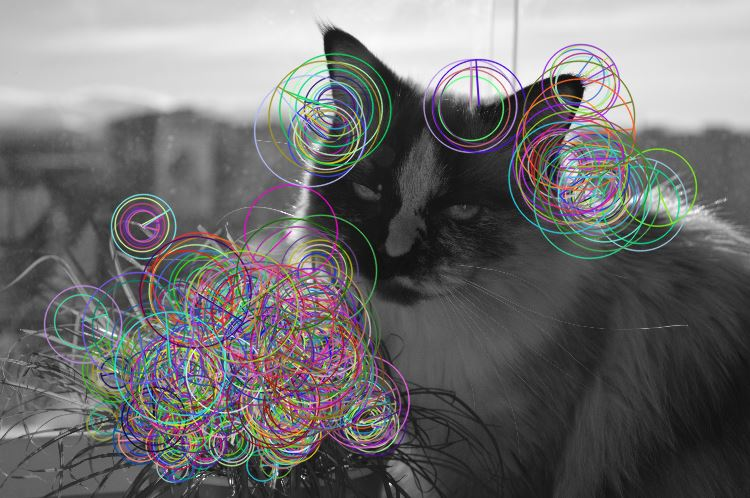
\includegraphics[width=0.65\textwidth]{Figures/orb/orb_example.jpg}
    \caption[ORB key-points and their orientation from an image of a cat]{ORB key-points and their orientation from an image of a cat.}
    \label{fig:orb_example}
\end{figure}

As an ORB descriptor, a variation on the BRIEF descriptor is used. The BRIEF descriptor is a vector of binary values. This allows for fast matching using a Hamming distance.

The descriptor values are computed by comparing random pairs of pixel intensities in a patch. The binary vector is based on the test defined as
\begin{equation}
    \tau(\boldsymbol{p};x,y)=
    \begin{cases*}
        1 & if $\boldsymbol{p}(x) < \boldsymbol{p}(y)$, \\
        0 & otherwise,
    \end{cases*}
\end{equation}
where $\boldsymbol{p}(x)$ is the pixel intensity of a patch $\boldsymbol{p}$ at a point $x$. The pairs of points $x$ and $y$ are from a random predetermined set
\begin{equation}
    \boldsymbol{S} =
    \begin{pmatrix}
        x_1 \dots x_n \\
        y_1 \dots y_n
    \end{pmatrix},
\end{equation}
where $n$ is the size of our descriptor. The BRIEF descriptor is defined as a vector of $n$ binary tests
\begin{equation}
    f_n(\boldsymbol{p}) \coloneqq \sum_{i=1}^{n} 2^{i-1}\tau(\boldsymbol{p};x_i, y_i).
\end{equation}

The steered version of the BRIEF descriptor, according to the orientation $\theta$ of the key-point, can be created by using a corresponding rotation matrix $\boldsymbol{R}_\theta$:
\begin{equation}
    \boldsymbol{S_\theta} = \boldsymbol{R}_\theta \boldsymbol{S}.
\end{equation}
The sets of pairs are precomputed in a lookup table for discretized $\theta$ in increments of $\frac{2\pi}{30}$ to improve speed. In the end, the steered BRIEF descriptor becomes
\begin{equation}
    g_n(\boldsymbol{p}, \theta) \coloneqq f_n(\boldsymbol{p}) | (x_i, y_i) \in \boldsymbol{S}_\theta.
\end{equation}
